\chapter{Cascade of Transducers}
\label{chap-cassys}

The general principle of a \textit{cascade of transducers} \index{cascade of transducer} is to apply several transducers, one 
after the other, onto a text to modify this text. For the system Unitex, a transducer is a graph. Such a system can be used to analyze a 
text in different ways: syntactic analysis, chunking, information extraction or simply to transform and/or prepare a text further treatments.

\bigskip
\noindent The prototype of the \textit{CasSys} \index{CasSys} system was created in 2002 at the LI 
( the laboratory of Computer science of the University of Tours) as part of Nathalie Friburger's PhD Thesis (\cite{reco-np-friburger02}). 
Later on, it was fully dedicated to named entity extraction. CasSys was generalized to allow any sort of work needing a cascade: throughout the years, 
 it was improved but never really integrated in Unitex, until the recent "Feder-R�gion Centre" project launched by Denis Maurel which resulted in the complete integration of CasSys in Unitex carried out by David Nott and Nathalie Friburger. 


\bigskip
\noindent A priori, the use of CasSys is roughly a succession of locate patterns eventually with special options and behaviors. 
In this chapter, we will explain how to create cascades of transducers and how to apply them. After that, we deals with details on what is very specific in CasSys.

%%%%%%%%%%%%%%%%%%%%%%%%%%%%%%%%%%%%%%%%%%%%%%%%%%%%%%%%%%%%%
\section{Applying a cascade of transducers with CasSys}
\label{section:applyCascade}

In the text menu, you can select the submesnu "Apply CasSys cascade..." (\ref{fig13-01}) which will open the CasSys window.
This submenu "Apply CasSys cascade" is active only if a text has previously been opened.

\begin{figure}[!htb]
 \centering
 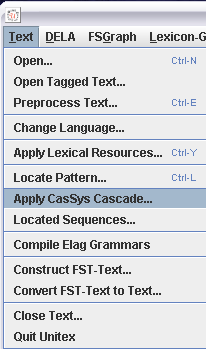
\includegraphics[width=5cm]{resources/img/fig13-01.png}
 \caption{"Text" menu of Unitex and submenu "Apply CasSys Cascade"}
 \label{fig13-01}
\end{figure}


\subsection{Creating the list of transducers}
\label{subsec:listTrans}

The list of transducers of a cascade is saved in a text file with the extension .csc (ex: mycascade.csc).

\bigskip
\noindent In order to create the list of transducers, click on the "new" button in the CasSys window. 
If you wish to modify an existing cascade, you can choose the file name of the cascade, then click on the "edit" button. 
These two buttons (edit or new) will open the "CasSys transducer configuration" window.

\subsection{Editing the list of transducers}
\label{subsec:editlistTrans}

The Cassys Transducer configuration window (\ref{fig13-03}) comprises three parts :

\begin{figure}[!htb]
  \centering
  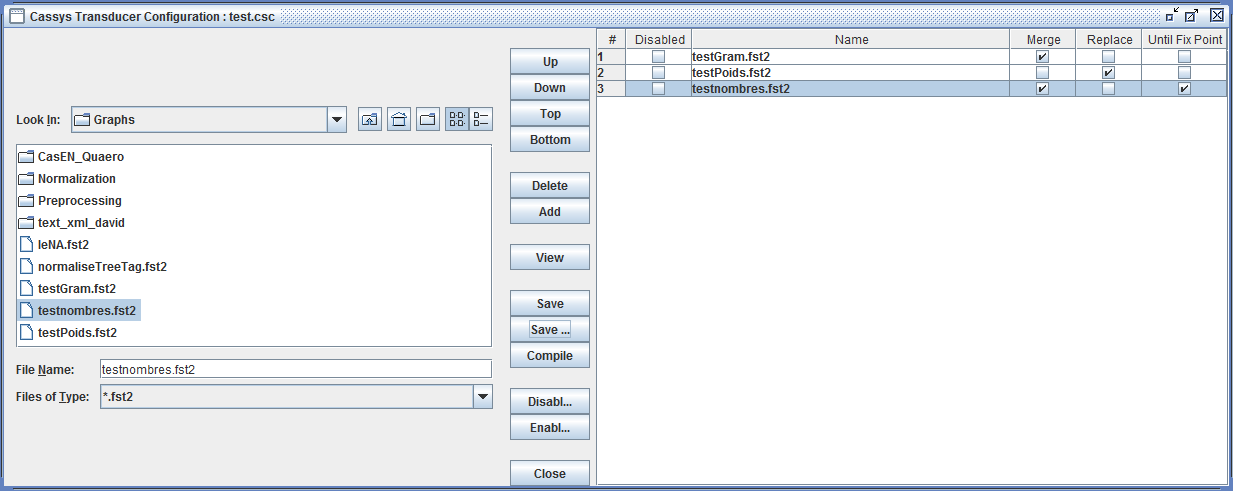
\includegraphics[width=14cm]{resources/img/fig13-03.png}
  \caption{Cassys Transducer configuration window with a list of transducers on the right hand side}
  \label{fig13-03}
\end{figure}

\begin{itemize}
	\item The left frame of the Cassys Transducer configuration window contains a file explorer in which you can select the transducers to add to the cascade. 
	The file explorer only displays fst2 files (all the graphs you want to place in the list of transducers must be compiled in fst2 format). 
	To edit the cascade, you must select the graphs in the file explorer in the left frame and drag and drop them into the right frame of the window.
	\item In the right frame, there is the list of transducers which is empty when
	creating a new cascade. The list of transducers is ordered: the first graph on the list is applied
	first, and the last graph on the list is applied last. Each transducer has
	several options :
		\begin{itemize}
		  \item \textbf{\# :} Rank of the transducer in the cascade
		  \item \textbf{Name :} The name of the transducer graph (with extension
		  \emph{fst2})
		  \item \textbf{merge :} Whether the transducer should be applied in merge
		  mode
		  \item \textbf{replace :} Whether the transducer should be applied in replace
		  mode
		  \item \textbf{disabled :} Whether the transducer should be disabled. 
		  \item \textbf{star :} Whether the transducer should be applied once or until
		  no change occur (see \ref{sub:AppWhiCon})
		 \end{itemize}
	 
	\item In the middle column, you will have buttons which are described below: 
		\begin{itemize}
			\item The "up"/"down"/"top"/"bottom" buttons are used to modify the order of the transducers on the list (it moves the selected transducer in the list); 
			"up" and "down" to move the selected transducer one line up or down, and "Top" and "Bottom" to move the selection to the top or to the end of the list.
			\item  The "delete" button permits to remove a selected transducer from the list of transducers. The "Add" button adds a transducer (previously selected in the explorer) onto the list. The "Add" button replaces the drag and drop actions described above. 
			\item The "View" button opens the selected graph either in the file explorer or in the list of transducers of the window. It is very useful to get a quick access to any transducer either to take a quick look at its content or to modify it.
			\item The "Save" button and "Save as" button permit to save the list of transducers. By default, the lists of transducers are stored in the CasSys folder of the current language (e.g. English/Cassys).
			\item The "Close" button closes the current window.
		\end{itemize}
\end{itemize}

\subsection{Sharing a cascade transducer list file}
\label{subsec:shareCascade}

In order to ease collaborating work within CasSys, a  simple export/import
transducers list file feature is provided.

To share a cascade list file, the following steps has to be fullfilled :
\begin{enumerate}
  \item \textbf{Export :} Select a cascade file and click the export button. (A
  ready to share file is created in the \texttt{/Cassys/Share} repository)
  \item Send the shared file to your colleague
  \item \textbf{Import :} Select the import file and click the import button.
  (A ready to use file is created in the \texttt{/Cassys} repository)
\end{enumerate}

\subsection{Launching a cascade}
\label{subsec:launchCascade}

The CasSys window (\ref{fig13-02}) displays the contain of the CasSys folder of the current language. It permits to choose 
the file containing the list of transducers to apply on the text. The displayed files are in a special file type "CaSCade configuration file" (.csc). 
When this list is chosen, you can click on the "Launch" button to apply the cascade.

\begin{figure}[!htb]
  \centering
  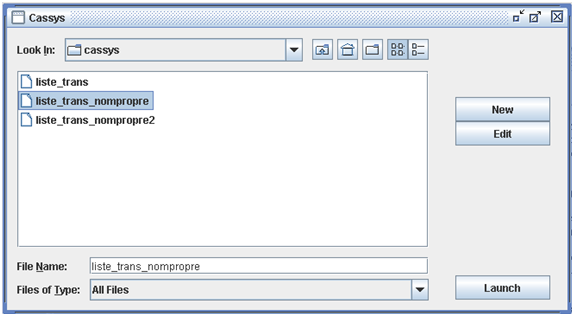
\includegraphics[width=10cm]{resources/img/fig13-02.png}
  \caption{CasSys Window to launch a cascade of transducers}
  \label{fig13-02}
\end{figure}


Any morphological dictionnaries added in your preferences is applied to your
graphs. This preferences may be edited from the main unitex frame (info -->
Preferences --> morphological dictionnaries).

\subsection{Displaying the results of a cascade}
\label{subsec:resultsCascade}

The result of a cascade is an index file (concord.ind), just as for the locate pattern operation. This index file contains all the sequences recognized using the restrictions imposed by the rules of unitex.

\bigskip
\noindent In order to display a concordance, you have to click on the "`Build concordance"' button (as described in Chapter \ref{chap-advanced-grammars}) 
in the menu "Text / Located sequences" (\ref{fig13-04} presents a sample of concordance of the results of a cascade recognizing named entities).
To create the file containing all the modifications of the cascade on the text, you have to click on "Modify text" in the "Located Sequences" window.
 The resulting file is a copy of the text in which the transducer outputs appear.

\begin{figure}[!htb]
  \centering
  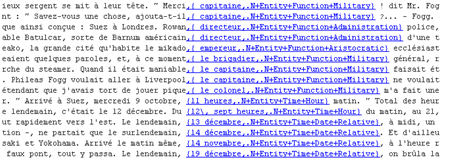
\includegraphics[width=14cm]{resources/img/fig13-04.png}
  \caption{Concordance of Cassys under Unitex}
  \label{fig13-04}
\end{figure}

%%%%%%%%%%%%%%%%%%%%%%%%%%%%%%%%%%%%%%%%%%%%%%%%%%%%%%%
\section{Details on Cassys}

In this section , we present details concerning the functioning of Cassys.

\subsection{Type of graphs used}

Cassys uses the compiled version of the graphs (the fst2 files).
Cassys can handle the local grammars (section 6.1) (syntactic graphs) presented in Chapter \ref{chap-advanced-grammars}. These grammars can use subgraphs, 
morphological filters and mode,and allow to refer to information in dictionaries. 
The grammars used in the cascade must follow the constraints of the grammars used in Unitex.


\subsection{Apply while concordance behaviour}
\label{sub:AppWhiCon}

Cassys may apply a transducer on a text while concordances are found. 

For
instance, consider the graph \ref{fig:AB->A} which recognizes \emph{AB} and
replaces it with \emph{A}. 

\begin{figure}[!htb]
  \centering
  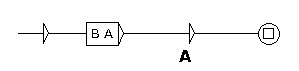
\includegraphics[width=6cm]{resources/img/AB_to_A.png}
  \caption{Transducer which modifies BA in A}
  \label{fig:AB->A}
\end{figure}

Consider the text \emph{B B B A A A}. \\

Applying the graph \ref{fig:AB->A} ont this text with emph{apply while
concordance behaviour} will have the following result :\\

\begin{tabular}{|l|cccccc|r|}
\hline
initial text  &B&B&B&A&A&A&\\
\hline
iteration 1 & &B&B&A&A&A& 1 concordance\\
iteration 2 & & &B&A&A&A& 1 concordance\\
iteration 3 & & & &A&A&A& 1 concordance\\
iteration 4 & & & &A&A&A& 0 concordance\\
\hline
\end{tabular} \\

During the three first iterations, a concordance is found, so the graph
re-applied on the resulting text. At the fourth iteration, no concordance is
found, so the graph is not re-applied.

\large{\textbf{Warning :}} Be aware of the risk of livelock when applying this
option. For example, a transducer which recognizes \emph{A} and replaces it with
\emph{A} would be caught in a livelock if applied on the example text.

\subsection{An xml-like output text for lexical tags}

As an output, the lexical tag format is transformed into an xml-like format.
This change is done in order to provide an easier-to-manipulate text to the end
user.
From this format, it is easier to apply transducers to get the output anyone
wants.\\

More precisely, The lexical tag has the following format :\\
\begin{tabular}{c}
\texttt{
\{forme.lemme,code1+code2:flex1:flex2\}}
\end{tabular}\\

The xml-like output of cassys has the following format :\\
\begin{tabular}{ll}
\texttt{<csc>}&\\
	&\texttt{<form>forme</form>}\\
	&\texttt{<lem>lemme</lem>}\\
	&\texttt{<code>code1</code>}\\
	&\texttt{<code>code2</code>}\\
	&\texttt{<inflect>flex1</inflect>}\\
	&\texttt{<inflect>flex2</inflect>}\\
\texttt{</csc>}&\\
\end{tabular}



\subsection{The Unitex rules used for the cascade}

In the cascade, each successive graph is applied following the unitex rules:
\begin{itemize}
	\item Insertion to the left of the matched patterns : in the merge mode, the ouput is inserted to the left of the recognized sequence.
	\item	Priority of the leftmost match : during the application of a local grammar, overlapping occurrences are all indexed. 
	During the construction of a concordance, all these overlapping occurrences are presentend but CasSys modifies the text with each 
	graph of the cascade : so it is necessary to choose among these occurrences the one that will be taken into account. To do that, the priority is given to the leftmost sequence.
	\item Priority of the longest match : in CasSys, during the application of a graph, it is the longest sequence 
	that will be kept.
	\item	Search limitation to a certain number of occurrences: in Cassys, this search is not limited : such a limitation has no sense in the use of CasSys. We allways index all utterances in the text.
\end{itemize}

\subsection{A special way to mark up patterns with CasSys}

The output of the transducers can be used to insert special information into texts, particularly to mark up the  recognized patterns: it is 
possible to use all the marks you want such as ( ), [], "", etc. or xml tags such as <xxx> </xxx>, but Cassys proposes a special way to 
mark up patterns, that offers some advantages and that we present here.  

\bigskip
\noindent Unitex splits texts into different sorts of tokens like the sentence delimiter {S}; the stop marker {STOP}, contiguous 
sequences of letters, lexical tags {aujourd'hui,.ADV}, etc. The lexical tag is used by CasSys in a special way. The lexical tag (between curly brackets) is normally used to avoid ambiguities (see explanation in section \ref{tokenization} and in section\ref{section-displaying-sentence-automata}). 
For example, in a text, if you have the token \emph{\{curly brackets,.N\}}, neither "curly" nor "brackets" will be recognized but the whole sequence 
"curly brackets". A lexical tag can contain complex lexical information like \emph{N+Pers+Hum:fs}.
In a graph, you can look for a lexical token using the lexical information it contains: for example, you can write \emph{<.N>} to search 
a noun, \emph{<.Pers+Hum>} for a human person or \emph{<.Pers>}. These lexical masks are explained in the Chapter Searching with Regular Expressions in section \ref{section-special-symbols}.
 
\bigskip
\noindent In Cassys, we use the lexical tag in a special way. A cascade of transducers is interesting to locate the island of certainty first. It is necessary for such a system to avoid that previously recognized patterns be ambiguous with patterns recognized by the following graphs. To do that, you can tag the patterns of your graphs surrounding them by \emph{\{} and \emph{,.tag1+tag2+tagn\}} in the outputs of the graph (where \emph{tag1, tag2, etc.} are your own tags).

\bigskip
\noindent To explain this behavior, here is a very simple example. The text on which we work is :

\emph{bac a b c cc a b b ba ab a b bca a b c abaabc}.

\bigskip
\noindent The graph grfAB (\ref{fig13-05}) recognizes the sequence \emph{ab} in the text and tags this sequence with the lexical tag \{a b,.AB\}. This graph is merged with the text and adds its outputs \emph{\{ }and \emph{,.AB\}} to the text. 

\begin{figure}[!htb]
  \centering
  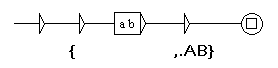
\includegraphics[width=6cm]{resources/img/fig13-05.png}
  \caption{The graph grfAB}
  \label{fig:fig13-05}
\end{figure}

\bigskip
\noindent The resulting text is : \emph{bac \{a b,.AB\} c cc \{a b,.AB\} b ba ab \{a b,.AB\} bca \{a b,.AB\} c abaabc}.

\bigskip
\noindent Now the pattern \emph{a b} is tagged \emph{AB}. A part (a or b alone) of this pattern cannot be recognized because of the tagging of \emph{a b}. 

\bigskip
\noindent After that graph, the cascade applies another graph named tagAB (\ref{fig13-06}) containing the lexical masks <AB>. It recognizes all the sequences lexically tagged by the previous graph.

\begin{figure}[!htb]
  \centering
  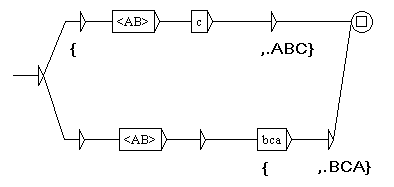
\includegraphics[width=10cm]{resources/img/fig13-06.png}
  \caption{The graph tagAB}
  \label{fig13-06}
\end{figure}

\bigskip
\noindent The resulting text is : \emph{bac \{\{a b,.AB\} c,.ABC\} cc \{a b,.AB\} b ba ab \{a b,.AB\} \{bca,.BCA\} \{\{a b,.AB\} c,.ABC\} abaabc}.

% \#M
% 2.0.0 6.0.0 \{\\\{a b\\,\\.AB\\\} c,.ABC\}
% 10.0.0 12.0.0 \{a b,.AB\}
% 20.0.0 24.2.0 \{a b,.AB\} \{bca,.BCA\}
% 26.0.0 30.0.0 \{\\\{a b\\,\\.AB\\\} c,.ABC\}

\bigskip
\noindent The concordance displayed by Unitex should be like in (\ref{fig13-07}). For programming reasons (ambiguities between characters in the curly brackets of the lexical tags), we have no option but to place backslashes $\backslash$ before all ambiguous characters ; that is why these symbols are protected with $\backslash$ in the concordance to avoid problems in Unitex. 

\begin{figure}[!htb]
  \centering
  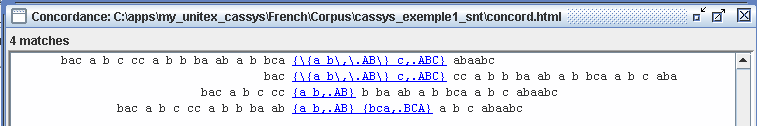
\includegraphics[width=15cm]{resources/img/fig13-07.png}
  \caption{The concordance resulting from this cascade}
  \label{fig13-07}
\end{figure}

\bigskip
\noindent This examples shows that the writing of graphs using the lexical tags created by preceeding graphs is very simple. The tags can overlap each other.

\subsection{Interest of a cascade of transducer}

Unitex grammars are known as Context free grammars and contain the notion of transduction derived from the field 
of finite state automata. A grammar with transduction (a transducer) is enabled to produce some ouput. 
Cassys is dedicated to the application of transducers in the form of a cascade.

\bigskip
\noindent Transducers are interesting because they allow the association of a recognized sequence to informations found in the outputs of the graphs. 

\bigskip
\noindent These outputs can:
\begin{itemize}
	\item	Be merged into the recognized sequence found in the text and appear in the resulting concordance or modified text. 
	\item	Replace the recognized sequence to modify the text. 
\end{itemize}

\bigskip
\noindent These two operations transform the text, add information inside the text for different purposes or modify it. The cascade can then be used for syntactic analysis, chunking, information extraction, etc. 

\bigskip
\noindent The advantage of a cascade is mainly that it is a good way to manage priority between patterns that you want to find in a text. If you know two ambiguous pattern, you can apply the less ambiguous pattern first.

\subsection{The longest pattern}

The heuristic of the longest pattern matching is applied to each transducer of the cascade. When a graph is applied to a text, several paths can be recognized
by the graph. 

\bigskip
\noindent If the graph arrives to its final state through several paths then it is the path that recognizes the longest pattern that is chosen. The longer
the pattern is, the less ambiguous it is.
If the transducer doesn't arrive to its final state then the recognizing step restarts on the next word of the text.

\bigskip
\noindent The longest pattern matching heuristic is interesting but if several paths of the same size are recognized there is still a problem; one of the paths will be chosen with no control on this choice for the user, meaning that the worst paht might well be chosen. A solution to that problem can be the creation of a cascade of transducer giving priority to a transducer among the list of transducers.

\bigskip
\noindent If a graph contains two paths that are ambiguous, one can create two graphs containing one path each. 
The first graph will contain the safest path, the second graph the least safe path.

\bigskip
\noindent Cassys keeps all the text created by each graph of the cascade. This can be useful to test, debug or check the different results of the cascade. It is possible 
to correct the errors on the order of the graphs or to find the errors in the writing of the graphs. A good idea is to place the name of the transducer recognizing a pattern in the outputs of the graphs: thanks to that, you can see in the final results the name of the graph by which a pattern is recognized. 

\subsection{Files resulting from CasSys}

If you apply a cascade on the text named example.txt, two folders are created: example\_snt and example\_csc.
The most important files produced in example\_csc are the results obtained by each graphs. These files are named according to the number of the graph which produced them (if the third graph finds a pattern, the result will be the file named example\_3.snt).
